\documentclass[11pt, conference]{IEEEtran}
\IEEEoverridecommandlockouts
\usepackage{amsmath}
\usepackage{amssymb}
\usepackage[english]{babel}
\usepackage{float}
\usepackage[margin=1in]{geometry}
\usepackage[utf8]{inputenc}
\usepackage[square,numbers]{natbib}
\usepackage{tikz}
\usepackage{titlesec}
\usetikzlibrary{automata,positioning}
\pagenumbering{gobble}
\bibliographystyle{plainnat}
\def
\BibTeX{{\rm B\kern-.05em{\sc i\kern-.025em b}\kern-.08em
    T\kern-.1667em\lower.7ex\hbox{E}\kern-.125emX}}
\titleformat{\section}
{\normalfont\Large\bfseries}{\arabic{section}.}{1em}{}
\titleformat{\subsection}
{\normalfont\large\bfseries}{\arabic{section}.\arabic{subsection}}{1em}{}
\titleformat{\subsubsection}
{\normalfont\normalsize\bfseries}{\arabic{section}.\arabic{subsection}.\arabic{subsubsection}}{1em}{}

\begin{document}

\title{Publisher/Subscriber Service}

\author{
	\IEEEauthorblockN{Xiao Xin}
	\IEEEauthorblockA{
		\textit{Stanford University} \\
		\textit{xxin@stanford.edu}
	} \\
	\and
	\IEEEauthorblockN{Chi Zhang}
	\IEEEauthorblockA{
		\textit{Stanford University} \\
		\textit{zcdirk@stanford.edu}
	}
}

\maketitle

\begin{abstract}
Publisher/Subscriber (Pub/Sub) is an asynchronous messaging-oriented service that serves as the backbone of contemporary distributed systems. In many cases it is used to decouple the functions of a massive monolithic application by aggregating multiple smaller yet more cohesive services. Being such a critical component to distributed systems, Pub/Sub services should also be scalable so it could fit the requirement of the services that depend on it. This project aims to replicate the functions of a pub/sub service with the capabilities to horizontally scale onto multiple machines to better serve the distributed systems it supports.

\end{abstract}

\section{Overview}
Intuitively, a Pub/Sub system has two components: publisher and subscriber. If a publisher knows what clients are its subscribers, messages will be delivered as requested. However, such design could be troublesome once the number of publishers and subscribers increases, total numbers of connection between publishers and subscribers increases exponentially, which would make the system highly coupled and barely manageable. To resolve the concern, broker, a middleware to decouple relations between publishers and subscribers, is introduced to the system.
	
	\begin{figure}[H]
	\centering
	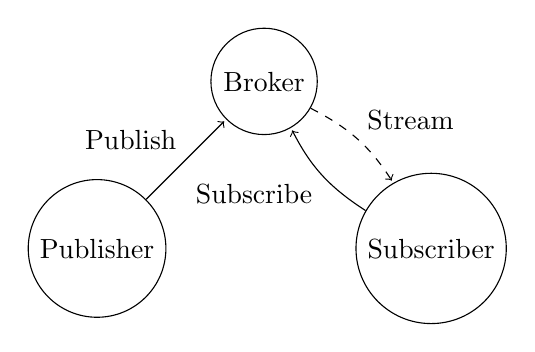
\begin{tikzpicture}[shorten >=1pt,node distance=3cm,on grid,auto]
		\node[state] (0) {Publisher};
		\node[state] (1) [above right=of 0]{Broker};
		\node[state] (2) [below right=of 1]{Subscriber};
		\path[->]
			(0) edge node {Publish} (1)
			(1) edge [bend left=15, dashed] node {Stream} (2)
			(2) edge [bend left=15] node {Subscribe} (1);
	\end{tikzpicture}
	\caption{Pub/Sub System Logical Model}
	\end{figure}

As the figure has shown, with broker in place, publisher and subscribers would only keep track of where the broker is and describe the action it wants to perform to it. The Pub/Sub service designed and implemented in this research serves as the broker in the logic model. It offers the following 2 APIs:

\begin{itemize}
  \item \textbf{Publish}: A client publishes a message of a certain topic to the broker, then the broker will tell the publisher whether the push is completed.
  \item \textbf{Subscribe}: Clients subscribe to topics from the broker, then the broker will push streams of messages under the requested topics to the subscribers.
\end{itemize}

Researchers started off with a primitive monolithic gRPC\citep{grpc} implementation of Pub/Sub on a single machine. Using it as a foundation, the developers then designed sidecar services to assist replication along with single-machine server. For different use cases, Pub/Sub service is implemented to scale up in the following modes:

\begin{itemize}
  \item Master-slave
  \item Leader election using Raft\citep{raft}
\end{itemize}

For each replication mode researchers applied multiple rounds of simulation and load testing using docker-compose\citep{docker-compose}. Each node in the cluster restricted to use 0.5 unit of CPU and 2GB of memory, the cluster is incrementally loaded to host 2000 clients simultaneously, and finally each client is supposed to receive around 20 messages each round and it is supposed to finish receiving all the messages within 1 second. 

The goal of this project is to compare how different replication schemes affects the performance of a distributed Pub/Sub system; hence, for simplicity all implementation only handles storage at memory level, no data is persisted any time in the lifecycle of a server process.


\section{Single-Machine}
The single machine implementation uses a thread-safe map internally to manage topics and subscribers. Each subscriber is put into its own thread\footnote{Service is implemented in Go\citep{golang}, where a thread is a go-routine.}. Every time a message is published, broker will first deliver the message to the subscriber threads of the message topic, and thereafter the message will be transported to clients in each thread. Figure 2 demonstrates the performance of a single-machine service throughout load-testing.

\begin{figure}[H]
	\centering
	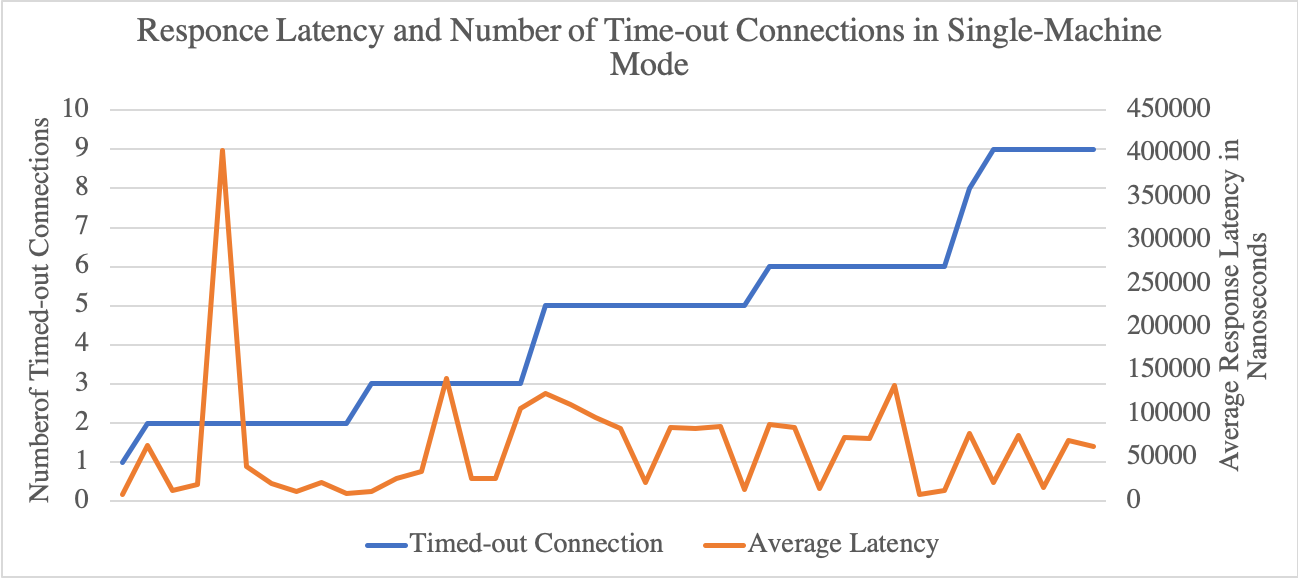
\includegraphics[scale=0.33]{figure/single_machine/performance.png}
	\caption{Single-Machine Performance}
\end{figure}

In average a single-machine service could finish a round of messages within 50 milliseconds. Several clients were blocked in the process and timed out; one possible reason could be that there is only one simulation process, so the client threads were locked, or maybe neglected, during user context switching. The issue should be negligible since the overall time-out rate is less than 0.5\%. The researchers later applied load-testing using the same setup to find out the maximum capacity of this implementation, and statistics showed that such a service could be handle 20000 clients with roughly 3\% timeout rate.

	
\section{Replication}
Although single-machine implementation could achieve acceptable performance, its capacity upper-bound is strictly limited by the computing power and storage space of the machine hosting it, and one must upgrade the hosting machine to scale up, which could be rather expensive. Following implementations provides ways to scale up the overall service capacities of the system by replicating and coordinating service process onto multiple machines. The machines involved in a distributed Pub/Sub systems are called \textbf{nodes}, and all nodes form a \textbf{cluster} that implements the functions of Pub/Sub systems.


\subsection{Master-Slave}
In master-slave cluster, a node is either a \textbf{master} or a \textbf{slave}. There is one and only one master in a cluster; master has no master to itself but slaves always have either a master or another slave as its master. Together all these nodes forms a tree-like topology with the root of the tree being the master of the cluster. 

In this mode each node has a sidecar service to assist master-slave replication.  Upon initiation, slaves post a request to its master's sidecar service to register as a known slave.

Masters and slaves handles subscribe action just as single machine implementation. Therefore, the system could easily increase reading throughput linearly by adding more nodes into the cluster. 

For publish, a slave would propagate the message to its master until the master of the cluster. Once received the message, the master would broadcast the message to all its slaves through their master-slave sidecar service, and then perform a publish action to its subscribers same as single-machine service. For slaves, they each manages a thread to listen to confirmed publish messages from its master, publish the message to its subscribers, and keep relaying the message to its slaves.

Since master-slave cluster forms a tree, one of the proposed design is to let nodes reserve a special topic for its slaves, and the slaves can just subscribe to the special topic to relay messages to their subscribers. However, the implementation is not adapted eventually for two reasons: first, developers have to introduce a guarding scheme to prevent users from interrupting system messages in reserved topics; second, the messages in reserved topic will have to be serialized at master to include metadata such as topic name and then deserialized at slaves, which introduces unnecessary operations. 

\begin{figure}[H]
	\centering
	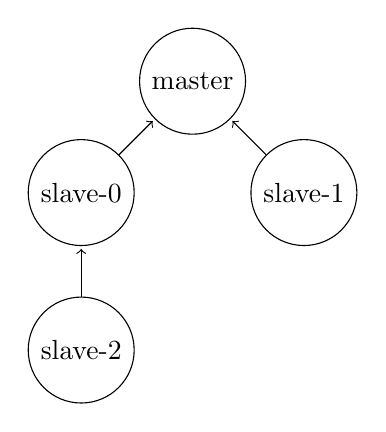
\begin{tikzpicture}[shorten >=1pt,node distance=2cm,on grid,auto]
		\node[state] (0) {master};
		\node[state] (1) [below left=of 0]{slave-0};
		\node[state] (2) [below right=of 0]{slave-1};
		\node[state] (3) [below=of 1]{slave-2};
		\path[->]
			(1) edge node {} (0)
			(2) edge node {} (0)
			(3) edge node {} (1);
	\end{tikzpicture}
	\caption{Master-Slave Cluster Topology}
\end{figure}
	
The researchers set up a cluster with 4 nodes organized as figure 4 for load testing. This organization includes all potential master-slave relation that could exists in master-slave mode, which could provide a more comprehensive demonstration of cluster performance.
	
\begin{figure}[H]
	\centering
	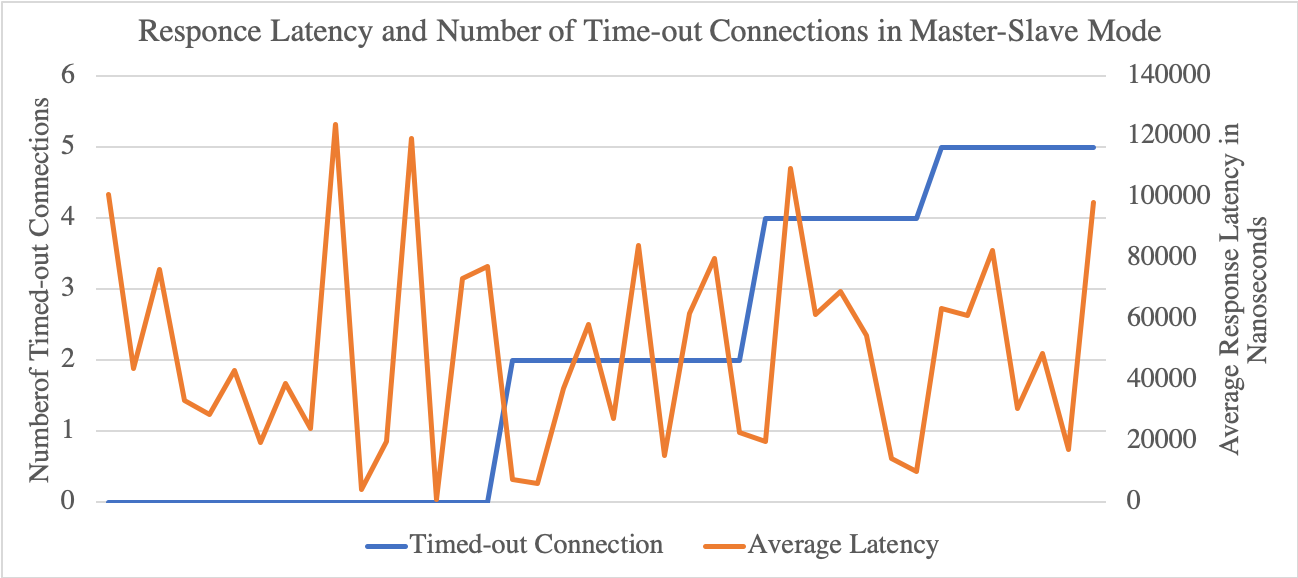
\includegraphics[scale=0.33]{figure/master-slave/performance.png}
	\caption{Master-Slave Performance}
\end{figure}

\begin{figure}[H]
	\centering
	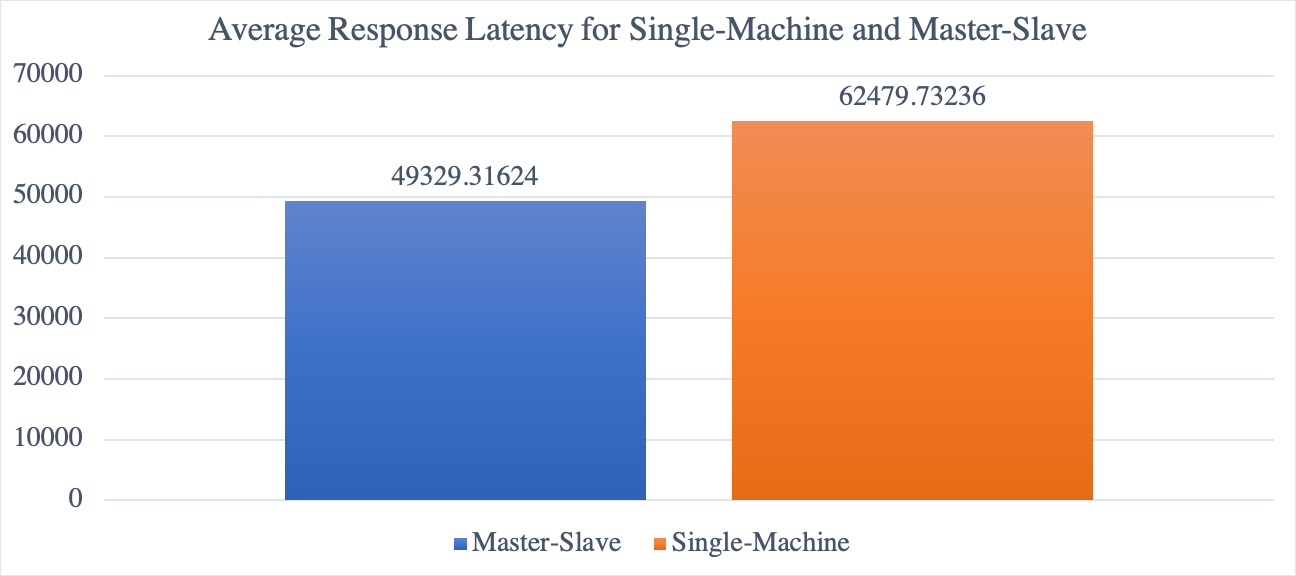
\includegraphics[scale=0.33]{figure/master-slave/response-latency.png}
	\caption{Single-Machine/Master-Slave average response latency}
\end{figure}

Figure 5 and 6 provide an overview of the capacity of master-slave Pub/Sub cluster. The statistics reflects here that, comparing to single-machine implementation, master-slave is slightly faster and has fewer timed out connections throughout the testing process. The testing program evenly distributed clients among nodes in the cluster, therefore causing each node  to handle only a quarter of load using the same amount of resources as the single-machine instance. The researchers actually expected master-slave architecture to be slower due to potential latency that may caused by message propagation through network. But since the testing cluster is hosted as containers sharing a virtual network on a single machine, the effect of network latency appears to become negligible. This finding could be helpful to users when they apply Pub/Sub in production, as they might be able to use master-slave mode to dispatch or collect data rapidly across regions with the leverage of reliable and performant network service, such as Google Could's high-performance premium tier network solution\citep{google-cloud-network}.

Master-slave's demonstrate decent potential, but its performance is in trade of reliability. If one node were to go down, all of the node's slaves and sub-slaves will lost sync with the rest the cluster at the same time. Besides, a master-slave cluster's performance is strongly correlated to its topology. If the cluster tree is too deep, or some of the nodes serving too many clients, the cluster's performance could be significantly affected. Only a balanced-tree of reasonable height with clients evenly distributed among nodes would make the cluster perform the finest. 
\

\subsection{Raft}
In master-slave mode, once one node fails, the failure would be cascaded all the way down to all of its slave-descendants. To resolve this concern, the Pub/Sub system must develop a way to find a replacement once its master went offline. Therefore, the researchers implemented a leader-election protocol on top of Pub/Sub system using Raft, which provides a less performant yet more reliable replication scheme for Pub/Sub. In this mode, all nodes are identified as \textbf{peer}, and the all could become the \textbf{leader} of the cluster once they win a majority of the ballots in leader election. The non-leader nodes are known as \textbf{follower}, and if they want to become the leader of the node they would first identity themselves as \textbf{candidate} to initiate an election. 


\subsubsection{Implementation basics}
On initiation, all the nodes start with the role of Candidate, and then start the election process. Each node will sleep a random time to avoid leader election conflict and then send out a leader-vote request if no others have done so. The node then collect the ballots from all the other peers, and once the node received majority vote grants, it will upgrade itself to leader. Upon upgrading to leader, the leader will send out initial RPC requests to all the other nodes to let others know about the leader.

\begin{figure}[H]
	\centering
	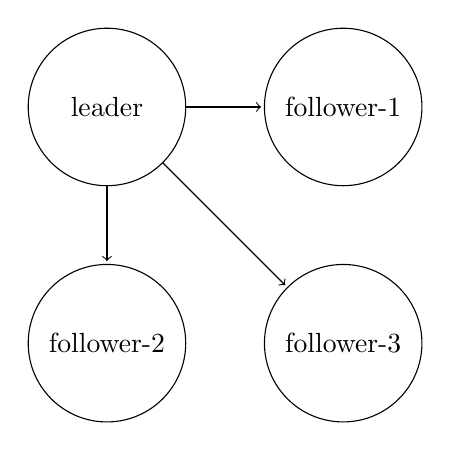
\begin{tikzpicture}[shorten >=1pt,node distance=2cm,on grid,auto,state/.style={circle, draw, minimum size=2cm}]
		\node[state] (0) {leader};
		\node[state] (1) [node distance=3cm,right=of 0]{follower-1};
		\node[state] (2) [node distance=3cm,below=of 0]{follower-2};
		\node[state] (3) [node distance=3cm,right=of 2]{follower-3};
		\path[->]
			(0) edge node {} (1)
			(0) edge node {} (2)
			(0) edge node {} (3);
	\end{tikzpicture}
	\caption{Raft Cluster Topology}
\end{figure}

After leader election, Raft cluster will be in a state shows in figure 7. The cluster will operates similarly to master-slave mode: all nodes in the system can handle subscribe request independently, and all publish requests will have to go through the leader. But to confirm the publish operation, leader must go through the some extra process to make sure the write request is accepted by most of the followers. Also, the leader needs to send out heartbeat request to let all the followers know that the leader is still active.



\subsubsection{Advantages}
Raft replication model has the following advantages over single machine model and master-slave model:

\begin{itemize}
  \item \textbf{Fault tolerant}: Single machine model cannot accept any crashes. Master slave machine can only accept slaves to crash. With Raft implementation, the service can still work fine as long as the majority of the nodes in the cluster are still alive. Also, after the crashed nodes recovered, they can catch up automatically and work as normal followers again.
  \item \textbf{Auto scalable}: In Raft model, Pub/Sub service allows the users to add new nodes into the cluster without rebooting the ones that already started. As long as the new node knows all the addresses of the existing nodes, it will send out a vote request on initiation. If the existing nodes receives a request with a candidate id that it has never seen, it will reply the vote request with fail, and then start a new connection with this node. This is pretty handy for the users, as they can add any number of new nodes whenever they want.
  \item \textbf{Log}: In single machine mode and master-slave mode, the messages are sent in the air, and will not be persisted in the log. While in Raft mode, as the leader needs to make sure all the followers are in the same state, nodes will persist all the message history in log. This makes it possible if the clients want to check the message history. Also, one more thing to point out here is after the crashed node recovers, it will catch up the logs and resend those messages the node received while it is down.
\end{itemize}



\subsubsection{Optimization}
In the process of development, the researchers tried different strategies to improve the efficiency. And finally decided to apply the following strategies to Pub/Sub service:

\begin{itemize}
  \item Discard the commit related fields and implementations in Raft. As we previously said, all implementation only handles storage at memory, there will be no data commit in the process.
  \item Create different threads for each heartbeat RPC and request vote RPC. In the first version, all the RPCs in the service are implemented in a blocking way so that the researchers can make sure all the processes come in sequence and are working as expected. However, in performance test, the researchers find that there maybe some nodes in the cluster are slower than the others and thus, the leader will be blocked by the slowest node in the cluster. Then the researchers decided to create a new thread for heartbeat request and vote request, which came out to improve the efficiency a lot. The researchers also tried to create a new thread for append entry request. But during tests, the subscribers may receive messages out of order, which is not acceptable. So the researchers decided to only create new threads for the sidecar transactions.
  \item Start the initial election immediately rather than wait for the timeout. In Raft implementation, the nodes only start a new election if it times out. This will be meaningless when we initialize the cluster. In this implementation, the node will send out a vote request once it finishes the setup and after a random waiting time. Which reduce the initialization time a lot.
  \item Wait a random time before send out a vote request. In the first implementation, the node will send out the vote request once it is timed out. However, during tests, the researchers found that the nodes may be a contention scenario during election process. So in the later version, the node will send out the vote request only after waiting a random time (between 0 and heartbeat timeout).
\end{itemize}

\subsubsection{Performance}
\begin{figure}[H]
	\centering
	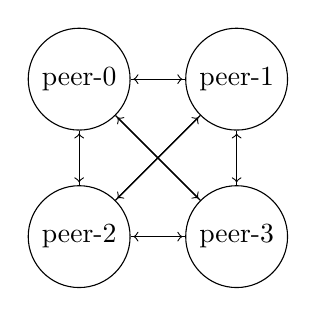
\begin{tikzpicture}[shorten >=1pt,node distance=2cm,on grid,auto]
		\node[state] (0) {peer-0};
		\node[state] (1) [right=of 0]{peer-1};
		\node[state] (2) [below=of 0]{peer-2};
		\node[state] (3) [right=of 2]{peer-3};
		\path[->]
			(0) edge node {} (1)
			(0) edge node {} (2)
			(0) edge node {} (3)
			
			(1) edge node {} (0)
			(1) edge node {} (2)
			(1) edge node {} (3)
			
			
			(2) edge node {} (0)
			(2) edge node {} (1)
			(2) edge node {} (3)
			
			
			(3) edge node {} (0)
			(3) edge node {} (1)
			(3) edge node {} (2);
	\end{tikzpicture}
	\caption{Raft Cluster Topology}
\end{figure}
In order to test the performance, the researchers organized a 4-node cluster for testing as figure 7. In additional to performance benchmarking, the researchers first applied a fault tolerance testing to validate leader-election by taking down a node in the cluster to see if the Pub/Sub system could still function. In most of the cases, leader nodes are taken down in order to observe how the cluster would re-elect a leader. All experiments suggests the leader re-elections were successful although some may cause significant latency during the process. Once the fault tolerance is confirmed to be successful, the researchers proceeded with performance benchmark.

	
\begin{figure}[H]
	\centering
	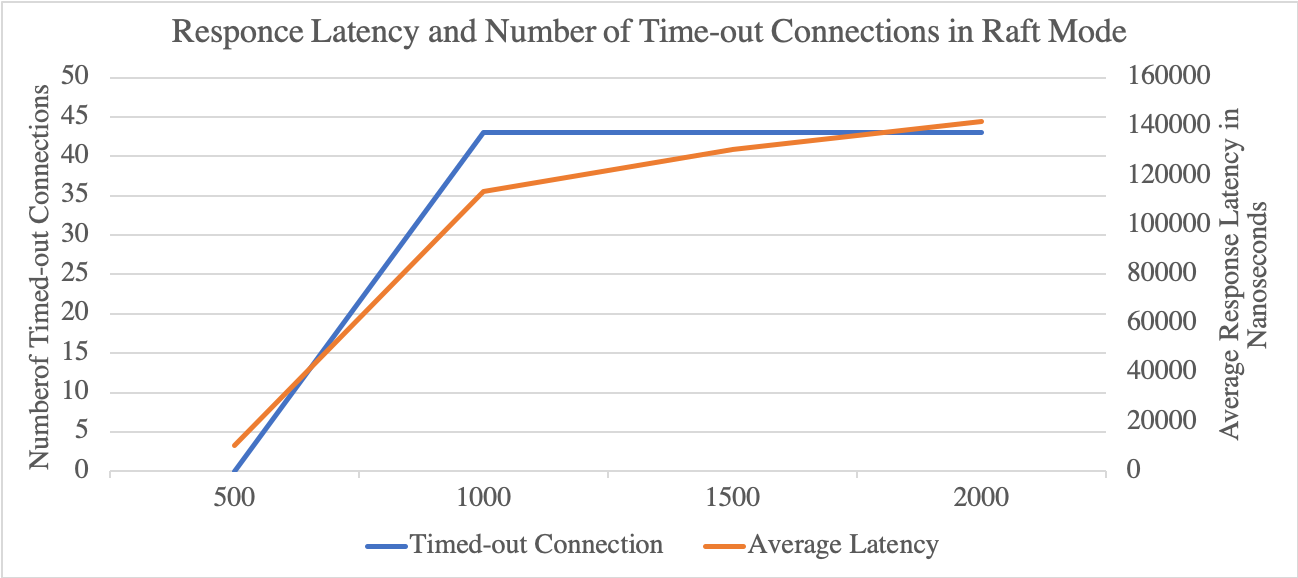
\includegraphics[scale=0.33]{figure/raft/performance.png}
	\caption{Raft Performance}
\end{figure}
	
\begin{figure}[H]
	\centering
	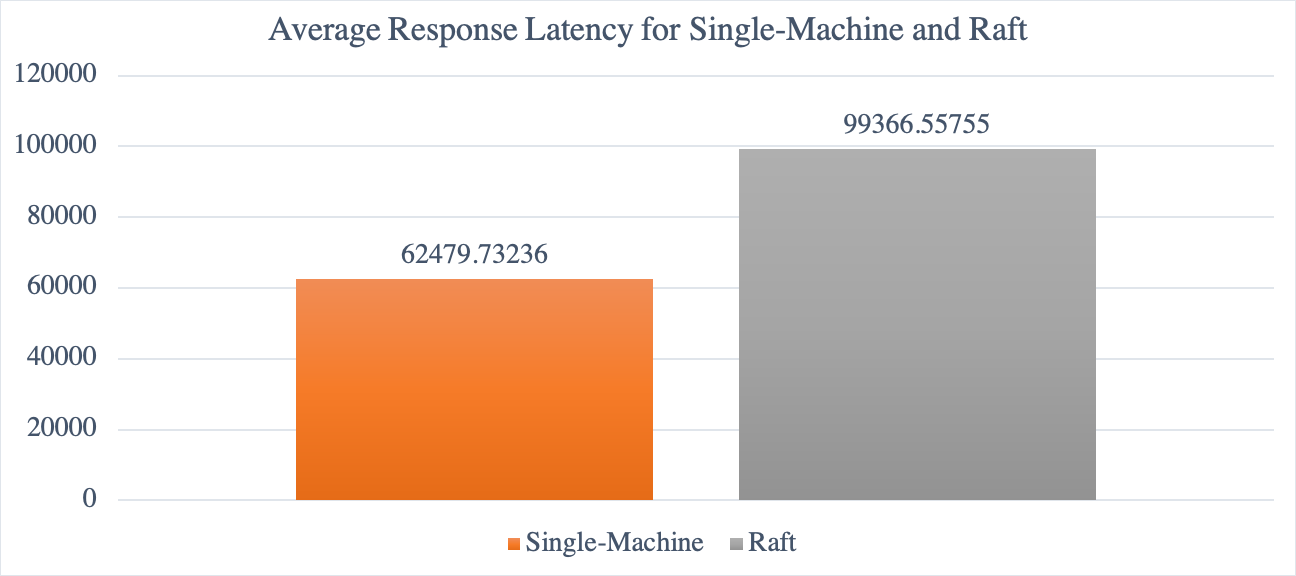
\includegraphics[scale=0.33]{figure/raft/response-latency.png}
	\caption{Single-Machine/Raft average response latency}
\end{figure}

Same in master-slave mode, the clients were evenly distributed onto each node in the cluster. However while testing, the researchers found that the system would be frequently stalled due to Raft-related heartbeat and synchronization operations, if the size of test increment were small. This effect can be cancelled out by extending heartbeat interval, but doing so would make the system behaving more like master-slave mode. Overall, the researchers decided to resolve the issue by increasing the test sample size in aim to reduce the total number of test iterations and internal leader elections. 

As the graph has shown, capacity-wise Raft-mode is still capable of hosting large number of clients. However, the average latency is over 50\% slower than that of a single machine, and timeout rate had also hiked.

\subsubsection{Future work}
There are also a few features proposed but not yet implemented due to time constraints. The researchers plan to leave them for future implementations:

\begin{itemize}
    \item \textbf{Authentication checking}: Currently, the implementation only allow one time subscribe, and the user don't need to provide any identification information. In the future, we may consider to add authentication checking in the service. Before subscriber subscribe a topic, the identification information is checked and the publisher may decide to publish the message to specific subset of subscribers that should have the permission to the message.
    \item \textbf{Client revive}: In current version, if a client lost connection with the server, it will miss the message in the meantime and have no way to retrieve those messages. After authentication checking is implemented, we may consider to store the last reply from the subscriber, and retry sending the messages after the subscriber lost connection. If the subscriber login again with the same account, then it should first received all the messages during the time that it is offline.
    \item \textbf{Message history query}: It will be handy if the subscribers can check all the message history based on the timestamp and topic. So that the client will not need to implement a client side log if they do need the history. We may also consider to implement this functionality.
\end{itemize}

\section{Conclusion}
Scaling remains one of the hardest problem in computer science and software engineering. Through this project, the researchers learned that different scaling approaches has its own comparative advantages: master-slave architecture could be one way to extend system performance; meanwhile leader election could be another way to improve system reliability. However, learning the advantages is not yet enough, the researchers also developed some thinking on how Pub/Sub and scaling could be further optimized in future.

First, the testing strategy adapted throughout the research mostly focused on subscribing side. Subscribe have to keep a long-lasting socket with Pub/Sub servers, but publish is more of a short-lived request but could take place frequently. Given current architectures, where all publish requests are essentially routed to a leader machine, when the publish traffic is at high level the performance of the system could be very different. Hence, how to scale up publish requests still remains an interesting problem that can be better addressed.

Second, after this project the researchers have the idea that the future of scaling solutions should be hybrid of multiple approaches. The essence of a distributed system is the topology it forms; therefore the system users should be able to manipulate such structure however they want to most efficiently solve the problems they need to tackle. Hence, if a distributed system solution could be configured to easily adapt multiple replication strategies, it is likely to be preferred by more users. While developing this system, the researchers attempted to extract the scaling functions as a set of standard interfaces, and the side-car services could just implement the interface. If this goal were to be achieved, the Pub/Sub system the researchers have designed could be able to provide multiple means of replication strategies on a single node. But this idea was eventually unapproachable due to the fact that Pub/Sub implementation needs to be written, such as rerouting publish requests to masters, in different replication strategies so that the strategy could work. In order to achieve the proposed idea, the Pub/Sub base API should be better designed so it has the flexibility to fit the requirements of replication strategies.

% TODO (zcdirk@)
% Talk about future action items 

\medskip
\bibliography{references}

\end{document}
